\chapter{Présentation du projet}
\section{Sujet}
Le problème à N-corps consiste à calculer le mouvement de  $N$ particules en connaissant leur position et leur vitesse initiales respectives.
Il s'agit donc de résoudre les équations du mouvement de Newton pour ces $N$ particules.
Le problème à N-corps est une simulation classique et importante pour l'astronomie, étant donné qu'il permet d'étudier la mécanique de corps céleste interagissant gravitationnellement.
Le problème à deux corps et le problème à trois sont  résolubles analytiquement. Pour $N>3$, il n'existe pas de résolution analytique, il faut donc utiliser des solutions approchées.

%inclusion d'une mage dans le document
\begin{figure}[!h]
\begin{center}
%taille de l'image en largeur
%remplacer "width" par "height" pour régler la hauteur
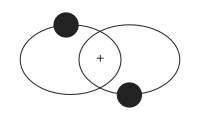
\includegraphics[scale=0.8]{presentation/two.png}
%légende de l'image
\captionsetup{hypcap=false}
\caption{Solution du problème à 2 corps \\
source : \url{https://femto-physique.fr}}
\label{fig1}
\end{center}
\end{figure}

\section{Objectif : résolution la plus efficace possible du problème à N-corps}

L'objectif du projet est donc de résoudre le plus efficacement possible le problème à n-corps afin de simuler des galaxies par exemple.
Pour cela, nous utiliserons des solutions approchées calculées à partir de différents algorithmes dont celui l'algorithme de Barnes-Hut. Nous étudierons également l'application de la parallélisation à notre programme.
En pratique, le projet consiste à continuer et améliorer un projet déjà bien entamé afin d'acquérir de nouvelles compétences en C++, sur les algorithmes hiérarchiques, en parallélisation et plus généralement en optimisation de code.

\section{Démarche}

%Un code C++ implémentant une interface graphique et les classes de base pour la résolution du problème nous a été fourni pour le projet.
%Nous allons dans un premier temps calculer la force qui s'applique à chaque particules à partir de la formule de l'interaction gravitationnelle. La position se calcule alors en utilisant un intégrateur numérique (Méthode d'Euler, saute mouton...).
%Dans un deuxième temps, nous utiliserons l'algorithme de Barnes-Hut pour le calcul des forces.
%Enfin, nous utiliserons la parallélisation multi-thread pour accélérer nos calculs.

Pour chaque particule, il est nécessaire de calculer la force gravitationnelle qui s'y applique puis d'utiliser un intégrateur numérique pour calculer sa position. Pour le calcul des forces, il est alors intéressant d'utiliser différents algorithmes notamment le calcul naïf et l'algorithme de Barnes-Hut. Pour l'intégration, il est possible d'utiliser la méthode d'Euler ou la méthode saute mouton.
Par la suite, il sera intéressant d'explorer les différentes possibilités d'optimisation, telle que la parallélisation multi-thread. 